\begin{titlepage}
  % HACK for two-sided documents: ignore binding correction for cover page.
  % Adapted from Markus Kohm's KOMA-Script titlepage=firstiscover handling.
  % See http://mirrors.ctan.org/macros/latex/contrib/koma-script/scrkernel-title.dtx,
  % \maketitle macro.
  \oddsidemargin=\evensidemargin\relax
  \textwidth=\dimexpr\paperwidth-2\evensidemargin-2in\relax
  \hsize=\textwidth\relax

  \centering

  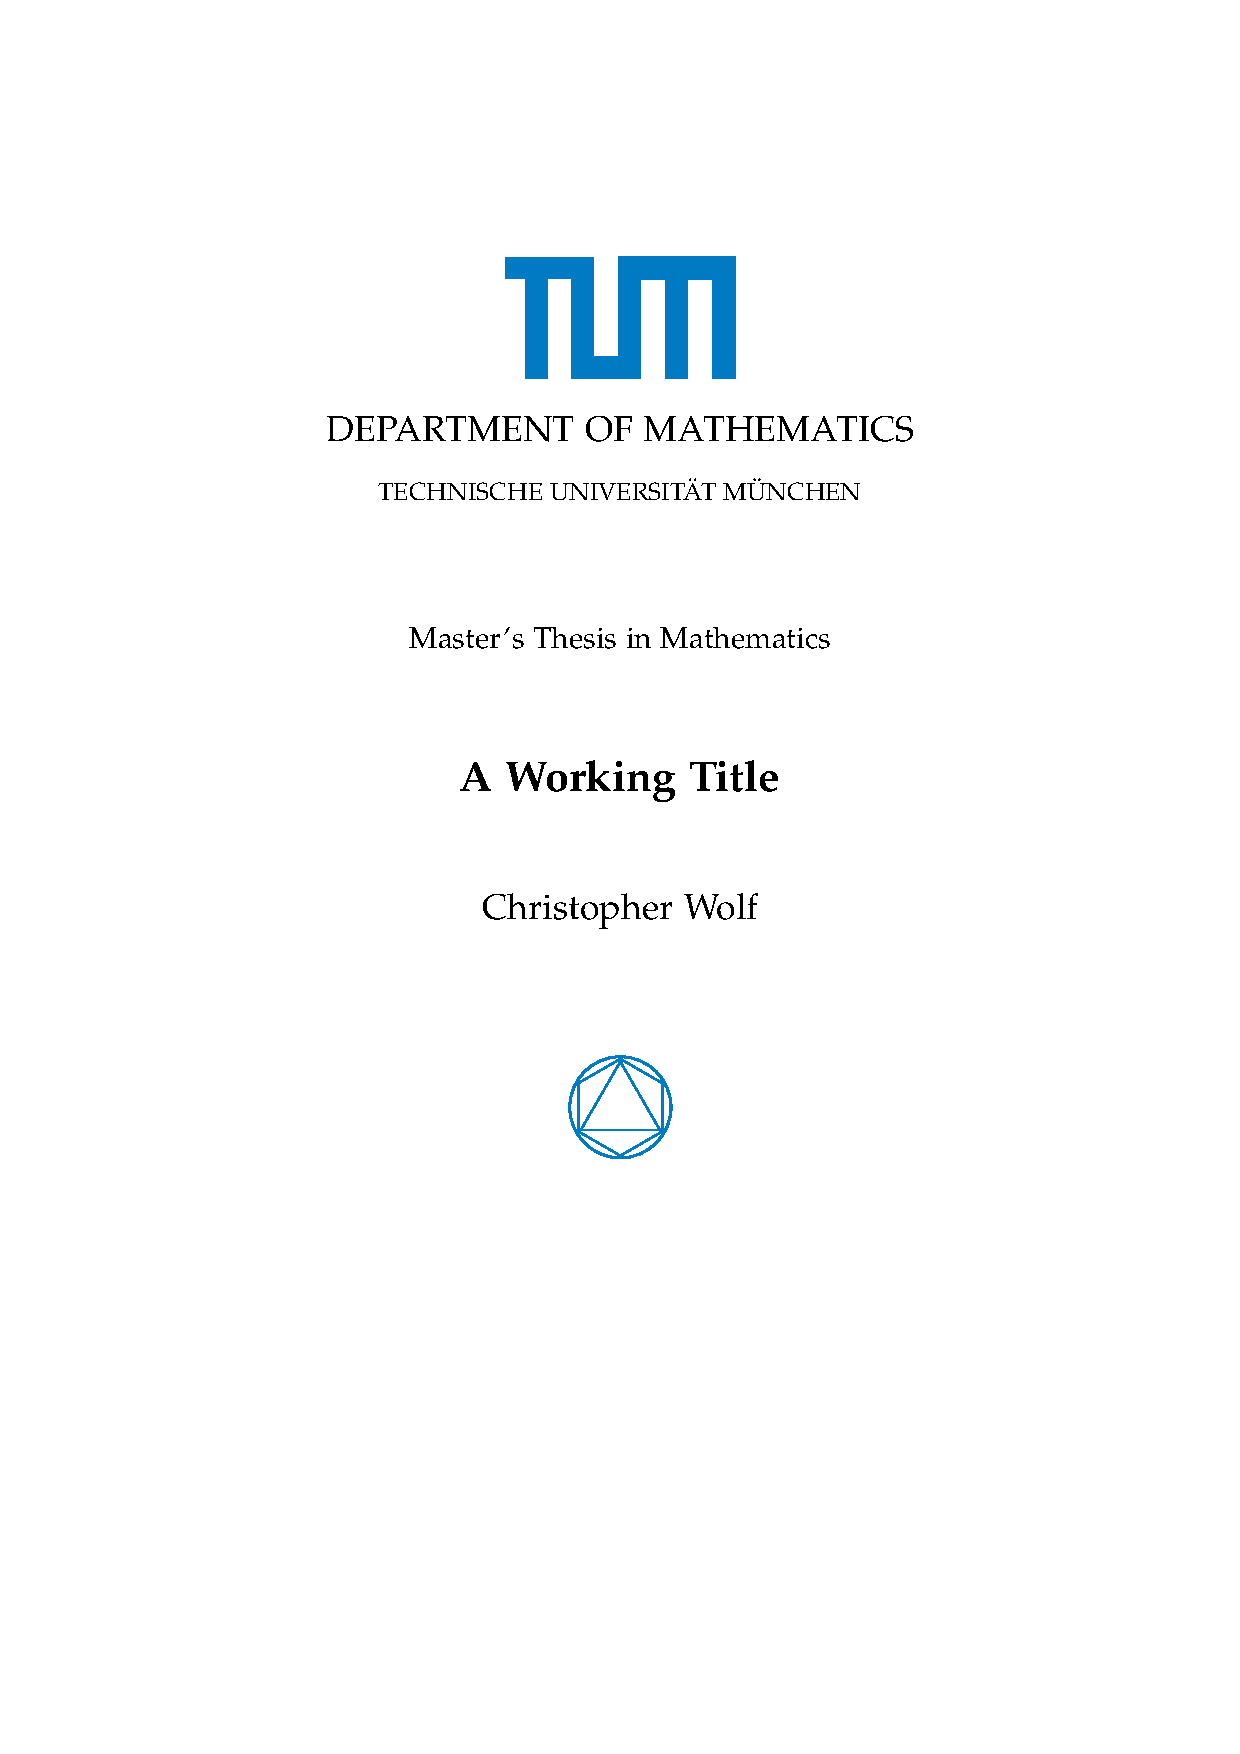
\includegraphics[width=40mm]{pages/tum}

  \vspace{5mm}
  {\LARGE\MakeUppercase{\getFacultyTUM{}}}\\

  \vspace{5mm}
  {\large\MakeUppercase{\getUniversityTUM{}}}\\

  \vspace{15mm}
  {\Large \getDoctypeTUM{}}

  \vspace{10mm}
  {\huge\bfseries \getTitle{}\par}

  \vspace{15mm}
  {\LARGE\getAuthor{}}

  \vspace{15mm}
  \begin{tabular}{l l}
    Supervisor: & \getSupervisorTUM{} \\
    Advisor: & \getAdvisorTUM{} \\
    Submission Date: & \getSubmissionDate{} \\
  \end{tabular}

  \vspace{10mm}
  \includegraphics[width=20mm]{pages/faculty}
\end{titlepage}
